\chapter{Confección del documento de tesis}

\label{Capitulo_25}
%----------------------------------------------------------------------------------------
\section{Primeras consideraciones}

Llamamos \textbf{tesina} a una tesis de grado, realizada en un lapso breve, estimado en un año. Es de esperar que los resultados sean también acotados en relación, por ejemplo, a los de una tesis de maestría o doctorado, pero no por ello, tales resultados van a resultar menores o poco interesantes. En lo que resta del texto, tesina o tesis se consideran equivalentes, pero siempre referido a un trabajo monográfico de grado.

La tesis es el documento que resulta del trabajo de investigación y desarrollo del estudiante, y al igual que ese trabajo, las tesis son muy personales, en lo que respecta al contenido y su estructura. De todas maneras, y al igual que sucede en todos los escritos, se deben respetar ciertas pautas \cite{melendrez2006como}.

%----------------------------------------------------------------------------------------
%----------------------------------------------------------------------------------------

\section{Estructura de una tesis}
\label{Estructura}
%----------------------------------------------------------------------------------------
\subsection{Fase Inicial}

Una tesis es, en su forma general, un libro que versa acerca del conocimiento, o desarrollo, alcanzado a partir de cierto trabajo, es así que se pueden encontrar algunas características comunes a cualquier libro que se adquiera en un librería:

\begin{itemize}
	\item \textbf{Portada}: debe contener el título  y la información del autor, incluyendo el lugar donde se realizó, nombre del director o supervisor y el año de presentación.
	\item \textbf{Cita}: Opcional, cuando se quiere mostrar alguna fuente de inspiración o modelo de vida, tanto personal, cívico o profesional.
	\item \textbf{Resumen}: El Resumen es una síntesis del trabajo, y por lo tanto debe tener una estructura similar, debe ser breve, buscando no exceder la página. Se debe escribir en forma sintética, refiriéndose a  los objetivos, la  metodología,  resultados principales y las conclusiones.
	\item \textbf{Agradecimientos}: Esta página es opcional, los agradecimientos  y reconocimientos se escriben a continuación. No forma parte del proyecto.
	
	\item \textbf{Indice} se compone por las siguientes listas:
	\begin{itemize}
		\item {\textit{Lista de Abreviaciones}, empleadas en la tesina, es de gran ayuda al lector, que le evita perder el tiempo en la búsqueda, en el texto, de una abreviación que no recuerda.}
		\item \textit{Glosario.}
		\item \textit{Índice de figuras.}
		\item \textit{Índice de tablas.}
		\item \textit{Índice General.} Lista y localización de los títulos de todas las secciones y sub-secciones pertenecientes al cuerpo de la tesis.
	\end{itemize}
	\item \textbf{Dedicatoria}: Esta página es opcional, y en ella se dedica el trabajo a personas tanto físicas como jurídicas.
\end{itemize}
%----------------------------------------------------------------------------------------
\subsection{Cuerpo de la tesis}

A partir de aquí, empieza el desarrollo de la tesis. La estructura difiere de tesis en tesis, pero una tesis bien escrita debe tener un hilo conductor, empezando por el problema y finalizando con las conclusiones y recomendaciones. En el medio, se leen el \textit{Objeto de Estudio}, los \textit{Objetivos} del trabajo de \ac{id}, las \textit{Tareas}, \textit{Metodología}, \textit{Resultados} y \textit{Discusión}.

Para profundizar sobre las relaciones existentes entre estas etapas, se puede consultar \cite{melendrez2006como}. Es importante notar que, de estas relaciones surge naturalmente la estructura de la tesis y esa estructura se vé en el Índice General. En lugar de dar inicio a la escritura en la introducción, Umberto Eco propone empezar por el índice, de manera tal que se pueda definir rápidamente el marco de trabajo \cite{eco2015write}.

\paragraph{La Discusión}
Este apartado merece una reflexión aparte. Puede  confundirse la \textit{Discusión} de un trabajo, con las \textit{Conclusiones} de mismo, o considerarlos equivalentes. No es así, son cuestiones diferentes, y  ambas son los apartados más importantes de la tesis. Por una parte la \textbf{Discusión} analiza los resultados obtenidos, busca la utilidad de ellos y los pone en contraposición con la literatura. Es el apartado donde se expone el  conocimiento generado, o el nuevo desarrollo tecnológico, y para ello, se contrasta con trabajos realizados por otros grupos del ámbito científico-tecnológico. Es posible encontrar los \textbf{Resultados} y la \textbf{Discusión} en un mismo capítulo.
Por otra parte, mediante las \textbf{Conclusiones}, que corresponden a la fase final de la tesis, se indican los logros en relación con los objetivos, problemas o preguntas planteadas, que se derivan de los resultados obtenidos.
%----------------------------------------------------------------------------------------

\subsection{Fase Final}

En la Fase Final de la tesis se encuentran las \textit{Conclusiones} y \textit{Recomendaciones}. En algunos casos, se las incluye en un único capítulo, pero conceptualmente deben abordarse en forma separada. Ibañez Brambila \cite{brambila2000manual} plantea sobre estos apartados que deben 
\begin{itemize}
	\item \textbf{Conclusión}: Representan un elemento esencial de la tesis puesto que es ahí donde se hacen constar los resultados obtenidos y la aportación de éstos en el ámbito estudiado. Aquí se da respuesta a los objetivos e hipótesis planteadas. La conclusión debe ser breve, respecto de la extensión del contenido, pero muy explícita, y donde “se manifiestan el valor del estudio, así como el dominio que se tiene del tema”
	\item \textbf{Recomendaciones}: Éstas se redactan después de las conclusiones. Se definen como sugerencias que se formulan con el propósito de indagar en el tema de investigación. Se puede recomendar otra dimensión del problema, o incluso otra forma  de  abordarlo.  Básicamente  se  trata  de  aportar  recomendaciones  para investigaciones futuras.
\end{itemize}

%----------------------------------------------------------------------------------------

\subsection{Referencias y Anexos.}

Terminando la tesis, se encuentran  los \textbf{Anexos}, con información que aporta y complementa a la tesis, pero que no tiene la relevancia para estar en el cuerpo principal, por algún motivo. Dentro de los anexos pueden encontrarse ejemplos de resultados, desarrollos teóricos extendidos, los cuales aparecen en el cuerpo de manera reducida, entre otras opciones. Por último se encuentra la lista de \textbf{Referencias}, es decir, la bibliografía sobre la cuál se basa y discute la tesis.

%----------------------------------------------------------------------------------------
%----------------------------------------------------------------------------------------

\section{Ejemplos de estructura}

En \ref{Estructura} se hizo un recorrido por las partes y apartados constitutivos de una tesis. A continuación se darán algunos ejemplos de estructuras, limitados al cuerpo de la tesina.
%----------------------------------------------------------------------------------------
\subsection{Ejemplo 1}
El ejemplo 1 es sumamente genérico, con una estructura que se puede encontrar en una tesis, pero también en los artículos científicos.

\begin{itemize}
	\item \textit{Capítulo 1: Introducción}
	\item \textit{Capítulo 2: Marco teórico y Estado del Arte}
	\item \textit{Capítulo 3: Objetivos}
	\item \textit{Capítulo 4: Metodología}
	\item \textit{Capitulo 5: Resultados}
	\item \textit{Capítulo 6: Discusión}
	\item \textit{Capítulo 7: Conclusiones}
	\item \textit{Capítulo 8: Recomendaciones}	

\end{itemize}
%----------------------------------------------------------------------------------------	
\subsection{Ejemplo 2}
El ejemplo 2 se extrajo de una tesis que fuera presentada para cumplir los requerimientos de la carrera de grado en Ciencias Biológicas, School of Science, Kathmandu University.

\begin{itemize}
	\item \textit{Capítulo 1: Introducción}
	\item \textit{Capítulo 2: Revisión Bibliográfica}
	\item \textit{Capítulo 3: Materiales y Métodos}
	\item \textit{Capítulo 4: Resultados y Discusión}
	\item \textit{Capítulo 5: Conclusión}
	\item \textit{Capítulo 6: Recomendaciones}
\end{itemize}
%----------------------------------------------------------------------------------------
\subsection{Ejemplo 3}
También se puede pensar en una estructura más adecuada al lugar y trabajo particular desarrollado

\begin{itemize}
	\item \textit{Capítulo 1: Introducción a los tópicos de la tesis}
	\item \textit{Capítulo 2: Teoría y estado de arte}
	\item \textit{Capítulo 3: Dispositivo experimental de Laboratorio}
	\item \textit{Capítulo 4: Detalles del experimento 1}
	\item \textit{Capítulo 5: Detalles del experimento 2}
	\item \textit{Capítulo 6: Discusión de los resultados experimentales}
	\item \textit{Capítulo 7: Conclusión y futuras direcciones de estudio}
	
\end{itemize}	

%----------------------------------------------------------------------------------------
%----------------------------------------------------------------------------------------

\subsection{Algunas reflexiones. }

(En construcción)
La tesis posee una estructura lineal, que está dada, según se comentó previamente,  por  su estructura, (capítulos, secciones, subsecciones). No obstante la información que esta contiene fluye entre sus partes. Cada capítulo requiere de los anteriores, y todos ellos vuelven, necesariamente, al primero, \emph{Estado del Conocimiento}. Ver figuta \ref{fig:flujo}.

\begin{figure}[th]
	\centering
	\includegraphics[width=0.6\textwidth]{Figuras/flujo}
	\captionsetup{margin=2cm}
	\caption[Flujo de lectura de la tesis]{La tesis, por  sobre su estructura lineal, necesita un flujo de información más complejo.  }
	\label{fig:flujo}
\end{figure}

Tenga en consideración, entonces,  que el desarrollo de la tesis, al igual que los trabajos realizados necesitan de todo el contenido. Por ejemplo, el Estado de Conocimiento es el paraguas sobre el que se realiza todo el trabajo, los resultados son consecuencia de la metodología, que a su vez tienen que ver con los Objetivos que se persiguen y debe poder relacionarse con el conocimiento existente. La Discusión existe gracias a los resultados, y en ella se estudian los nuevos descubrimientos en relación a lo que se sabe, considerando las condiciones que impone la metodología. Todo lleva a las conclusiones del estudio, y a el camino a seguir que se recomienda. 
%----------------------------------------------------------------------------------------
%----------------------------------------------------------------------------------------

\section{Características y convenciones de la tesis}\label{Convenciones}

Para aprovechar al máximo esta plantilla, existen algunas convenciones que tal vez desee seguir.

Una de las cuestiones más importantes, y más difíciles de controlar en un documento tan largo, como una tesis, es la coherencia. Usar ciertas convenciones y formas de hacer las cosas, como usar una lista de tareas, facilita el trabajo. Por supuesto, esto es opcional y puede adoptar su propio método.

%----------------------------------------------------------------------------------------

\subsection{Formato de Impresión}

Esta plantilla se configura para un papel A4, que es el tamaño estándar en Argentina y es el requerido en la presentación de la tesis. 
 
La plantilla está diseñada para impresión simple,  en una cara de la hoja. Se declara al principio del archivo \file{tesina.tex} el formato de la tesina \emph{report}:
\begin{verbatim}
	\documentclass{report}
\end{verbatim}

y el ajuste de página y  márgenes, 
\begin{verbatim}
	\usepackage[paper=a4paper,top=2in, bottom=1.5in, left=1in, right=1in]{geometry}
\end{verbatim}

 Para las tesis que se impriman, es preferible un formato de impresión doble faz, imprimiendo en el anverso y el reverso de las hojas, para ello comente las dos primeras líneas de código y des-comente la línea 
\begin{verbatim}
	\documentclass[twoside]{report}.
\end{verbatim}


Los encabezados de las páginas contienen el nombre del capítulo en el lado interior. y el número de página en el lado exterior (por lo que es fácil desplazarse hasta la página que desea).

El texto está configurado en 11 puntos por defecto con un espacio de una sola línea, nuevamente, puede ajustar el tamaño y espaciado del texto si lo desea, o necesita, usando las opciones. Para ello al comienzo de \file {main.tex}, se encuentra el bloque \emph{CONFIGURACIÓN INTERLINEA}.


%----------------------------------------------------------------------------------------
\subsection{Seccionado y Subseccionado}


Debes dividir su tesis en secciones y subsecciones de un tamaño adecuado para una correcta comprensión del texto. En la compilación, \LaTeX{} genera automáticamente una tabla de contenidos al compilar  todos los comandos \verb|\chapter{}|, \verb|\section{}| y \verb|\subsection{}| que escribe en el código fuente de su tesis.

La tabla de contenido solo debe enumerar las secciones en tres (3) niveles. Un \verb|\chapter{}| es el nivel cero (0). Una \verb|\section{}| es el nivel uno (1) y por lo tanto una \verb|\subsection{}| es el nivel dos (2). En su tesis es probable que incluso emplee \verb|\subsubsection{}|, que es el nivel tres (3).

%----------------------------------------------------------------------------------------
\subsection{Referencias}


El paquete \code{bibtex} se usa para formatear la bibliografía e insertar referencias como la siguiente \verb*|\cite{Referencia1}|: \cite{Referencia1}. Para simplificar se emplean las opciones por defecto de \code{bibtex}, las citas se organizan de acuerdo al orden de aparición en el cuerpo de la tesis. Las referencias múltiples están separadas por comas (por ejemplo, \cite{Referencia2, Referencia1}).

Las referencias científicas deben ir \emph{antes} del signo de puntuación si lo hay. Lo mismo ocurre con las notas al pie \footnote{Como esta nota al pie, aquí abajo en la parte inferior de la página.}. Puede modificar esto, pero lo más importante es mantener la convención consistente a lo largo de la tesis. Las notas al pie de página deben ser oraciones completas y descriptivas (comenzando con una letra mayúscula y terminando con un punto).

Existen otros paquetes que complementan a \code{bibtex} o \code{biblatex}, como por ejemplo \emph{natbib}, o que los reemplazan como \emph{biber}, ofreciendo mayores funcionalidades. Puede emplear el paquete de su preferencia.


%----------------------------------------------------------------------------------------









\section{Bienvenid@ y Gracias}
Bienvenida/o a esta plantilla de tesis en \LaTeX{}. Una plantilla simple de usar, para escribir su tesis usando el sistema de tipografía \LaTeX. 

Si va a escribir una tesis técnica o matemática, es recomendado realizarla en \LaTeX{}, de manera tal de concentrar los esfuerzos en lo esencial, sin preocuparse por cuestiones de formato, ni acceso a determinado procesador de textos.

\LaTeX{} puede componer fácilmente documentos de forma profesional que se ejecutan en cientos o miles de páginas. Con comandos de marcado simples, establece automáticamente en tabla de contenido,  márgenes, encabezados y pies de página, mantiene el formato consistente y atractivo. Una de sus principales fortalezas es la forma en que pueden componer fácilmente  fórmulas  matemáticas, incluso las expresiones más \emph{complejas}. Si esas ecuaciones son  problemas matemáticos  horriblemente retorcidos y difíciles, que solo pueden resolverse en una supercomputadora, al menos puede contar con \LaTeX{} para que se vean lindos.


%----------------------------------------------------------------------------------------
\section{Aprendiendo \LaTeX{}}

\ LaTeX {} no es un programa \textsc{wysiwyg} (What You See is What You Get - Lo que ve es lo que obtiene), a diferencia de los procesadores de texto como Microsoft Word o Pages de Apple. En cambio, un documento escrito para \LaTeX{} es en realidad un archivo de texto plano, simple, \emph {sin formato}. Para asignar formatos a lo escrito, se le dice a \LaTeX{}, cómo se quiere el formato en el documento terminado, escribiendo comandos simples entre el texto, por ejemplo, si quiere usar \emph{texto en cursiva para enfatizar}, se escribe el comando \verb | \emph{texto} |  con el texto que se quiere enfatizar  entre las llaves. Esto significa que \LaTeX{} es un lenguaje de \textit{marcado}, con cierto parecido  al HTML.



\subsection{Una (no tan corta) Introducción a \LaTeX{}}

Si es nuevo en \LaTeX{}, hay un libro electrónico muy bueno, disponible gratuitamente en línea como un archivo PDF, llamado \textit {The Not So Short Introduction to \LaTeX{}}. El título del libro suele acortarse a  \emph{lshort}. Puede descargar la última versión (ya que se actualiza ocasionalmente) desde aquí:

\url{http://mirrors.ctan.org/info/lshort/spanish/lshort-a4.pdf}

Se recomienda tomar un poco de su tiempo para aprender a usar  \LaTeX{} creando varios documentos pequeños de "prueba" u observando de cerca algunos ejemplos. Hacer el esfuerzo ahora significa que no estará atrapado aprendiendo el sistema cuando lo que \emph{realmente} necesita hacer es escribir su tesis.


\subsection{Una Guía Corta de Matemáticas para \LaTeX{}}

Si está escribiendo una tesis técnica o matemática, es posible que desee leer el documento de la AMS (American Mathematical Society) llamado \textit{A Short Math Guide for \ LaTeX {}}. Se puede encontrar en la dirección:
\url {https://ctan.dcc.uchile.cl/info/short-math-guide/}

Algunos ejemplos de ecuaciones, pueden ser \emph{en la línea}, escribiendo \verb*|$\int f(\alpha)~d\alpha$| obtendrá la ecuación en línea  $\int f(\alpha)~d\alpha$. Note que la ecuación se escribe entre \verb|$| y \verb|$|. La misma ecuación puede centrarse en la página escribiéndola entre \verb|$$| y \verb|$$|. $$\int f(\alpha)~d\alpha$$. No es la única forma de ingresar ecuaciones,  por ejemplo,

\begin{lstlisting}[basicstyle=\small,tabsize=4]
	\begin{gather}
		si ~ \not ~  C(s,a,a') < \bar{R} \tau  \Rightarrow ~  \Bigg \{ 
			{\begin{matrix}
				a \rightarrow  \{a,a'\} ~ en ~ s  \\
				sino \\
				\{a,a'\} \rightarrow a ~en~ s
			\end{matrix}}
	\end{gather}
\end{lstlisting}
 
 devuelve como resultante:
 
 \begin{gather}
 	si ~ \not ~  C(s,a,a') < \bar{R} \tau  \Rightarrow ~  \Bigg \{ 
 		{\begin{matrix}
 			a \rightarrow  \{a,a'\} ~ en ~ s  \\
 			sino \\
 			\{a,a'\} \rightarrow a ~en~ s
 		\end{matrix}}
 \end{gather}

Otro ejemplo, 

\begin{equation}
	\label{eq: gate}
	G(t) = \frac{t}{\tau_{ampa}} e^{-\frac{t}{\tau_{ampa}} } ~H(t)
\end{equation}

en este último ejemplo \ref{eq: gate}, se agregó un \emph{label}  para hacer referencia a la ecuación en el texto. El código para declarar la ecuación \ref{eq: gate} es: 

\begin{lstlisting}[basicstyle=\small,tabsize=4]
	\begin{equation}
		\label{eq: gate}
		G(t) = \frac{t}{\tau_{ampa}} e^{-\frac{t}{\tau_{ampa}} } ~H(t)
	\end{equation}
\end{lstlisting}
 

Es muy grande la diversidad de símbolos matemáticos, los cuales se pueden encontrar fácilmente buscando en la web, por ejemplo \url{http://math.mit.edu/~dspivak/files/symbols-all.pdf} ó también \url{http://www.sunilpatel.co.uk/latex-type/latex-math-symbols/}

%----------------------------------------------------------------------------------------
\subsection{Una guía corta sobre Tablas}

Las tablas son una forma importante de mostrar sus resultados, a continuación se muestra una tabla de ejemplo que se generó con este código:

{\small
	\begin{lstlisting}[basicstyle=\small,tabsize=4]
		\begin{table}
			\caption{Los efectos de los tratamientos X e Y en los cuatro grupos estudiados.}
			\label{tab:tratamientos}
			\centering
			\begin{tabular}{l l l}
				\toprule
				\tabhead{Grupos} & \tabhead{Tratamiento X} & \tabhead{Tratamiento Y} \\
				\midrule
				1 & 0.2 & 0.8\\
				2 & 0.17 & 0.7\\
				3 & 0.24 & 0.75\\
				4 & 0.68 & 0.3\\
				\bottomrule\\
			\end{tabular}
		\end{table}
	\end{lstlisting}
}

\begin{table}
	\caption{Los efectos de los tratamientos X e Y en los cuatro grupos estudiados.}
	\label{tab:tratamientos}
	\centering
	\begin{tabular}{l l l}
		
		\tabhead{Grupos} & \tabhead{Tratamiento X} & \tabhead{Tratamiento Y} \\
		
		1 & 0.2 & 0.8\\
		2 & 0.17 & 0.7\\
		3 & 0.24 & 0.75\\
		4 & 0.68 & 0.3\\
		
	\end{tabular}
\end{table}

Puede hacer referencia a tablas con \verb|\ref{<etiqueta>}| donde la etiqueta se define dentro del entorno de la tabla. Consulte \file{cap2.tex} para ver  ejemplos de etiquetado y citas (por ejemplo, el correspondiente a esta Tabla ~ \ref{tab:tratamientos}).

%----------------------------------------------------------------------------------------

\subsection{Una guía corta sobre Figuras}

Es de esperar que haya figuras en su tesis , y que deben localizarse en la carpeta \emph{Figuras}. Se pueden emplear formatos pdf, jpg and png. Una forma de insertar figuras en su tesis es usar una plantilla de código como la siguiente:

\begin{lstlisting}[basicstyle=\small,tabsize=4]
	\begin{figure}
		\centering
		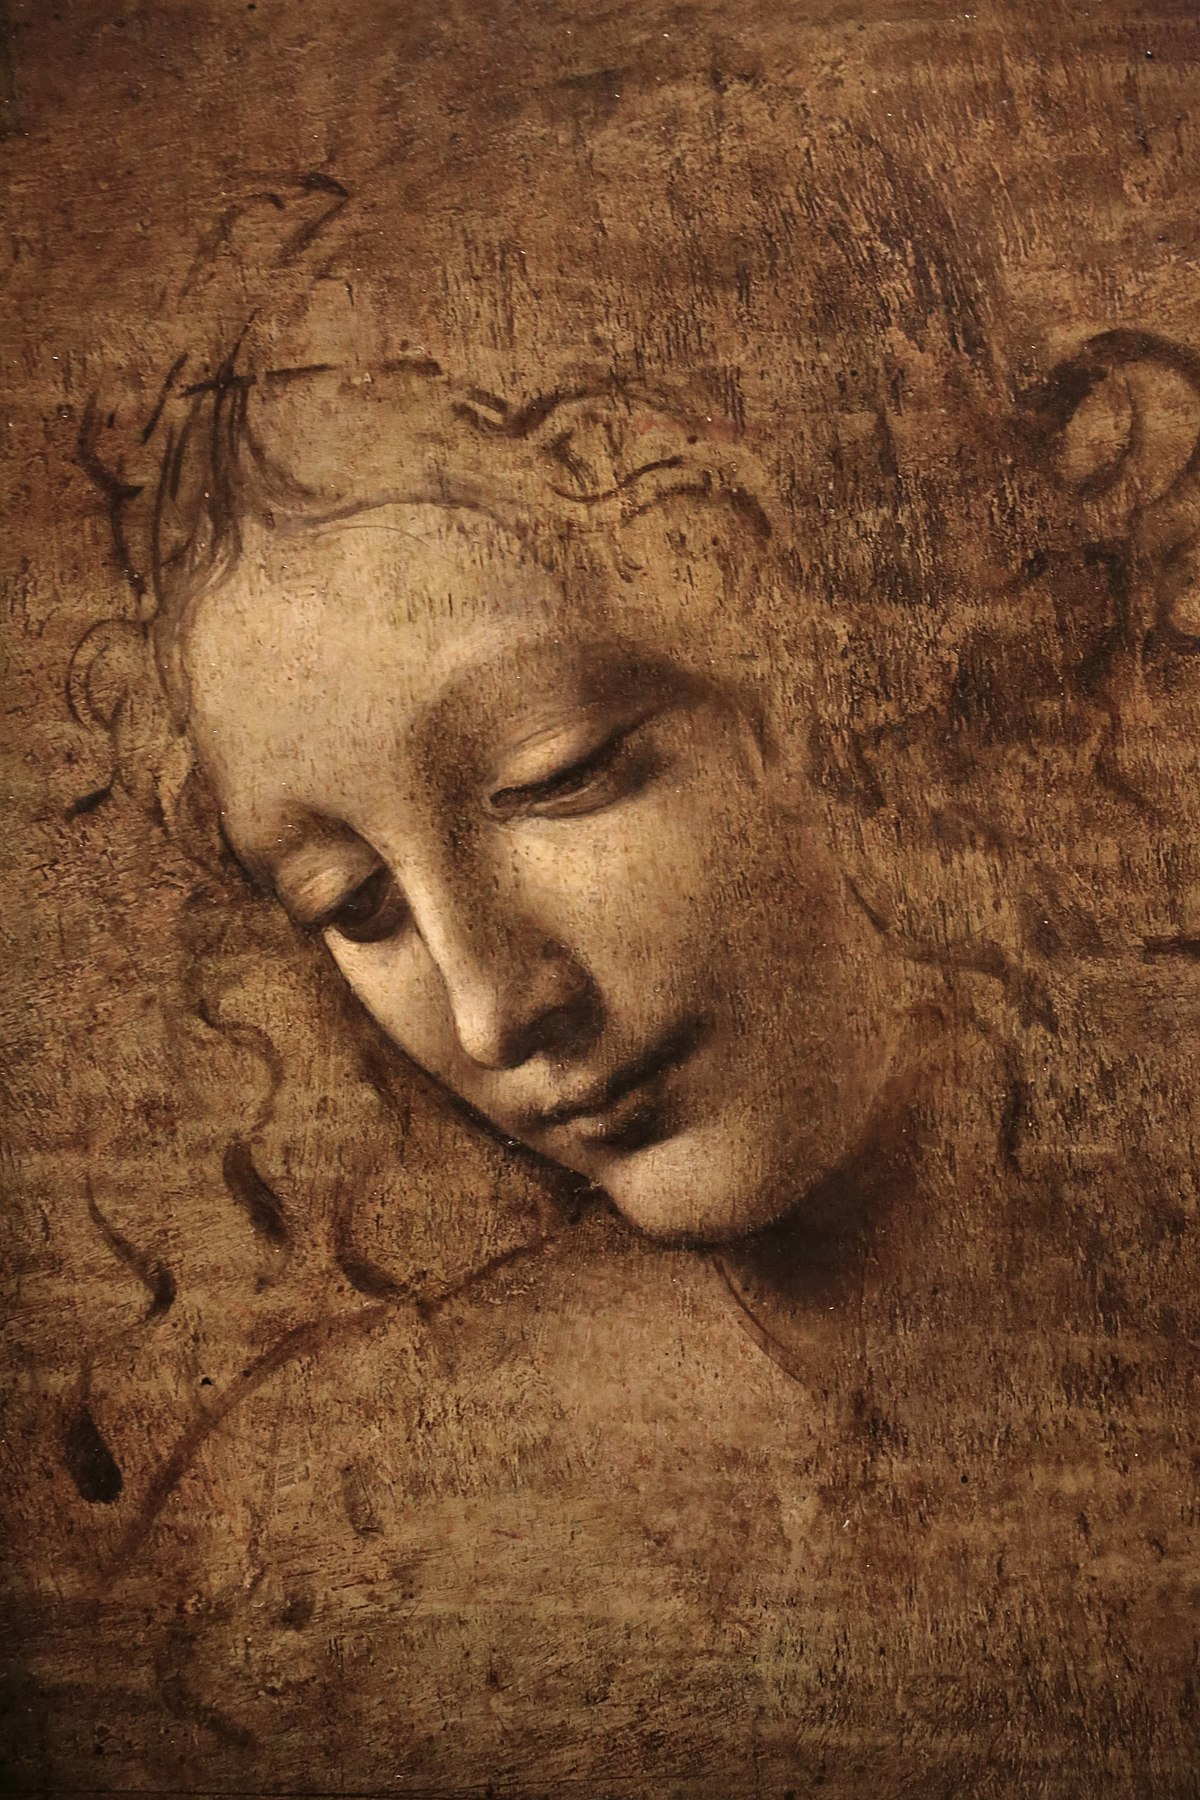
\includegraphics[width=0.6\textwidth]{Figuras/scapigliata}
		\captionsetup{margin=4cm}
		\caption[La Scapigliata]{La Scapiliata, una pintura al oleo sin ....}
		\label{fig:Scapigliata}
	\end{figure}
\end{lstlisting}


\begin{figure}[th]
	\centering
	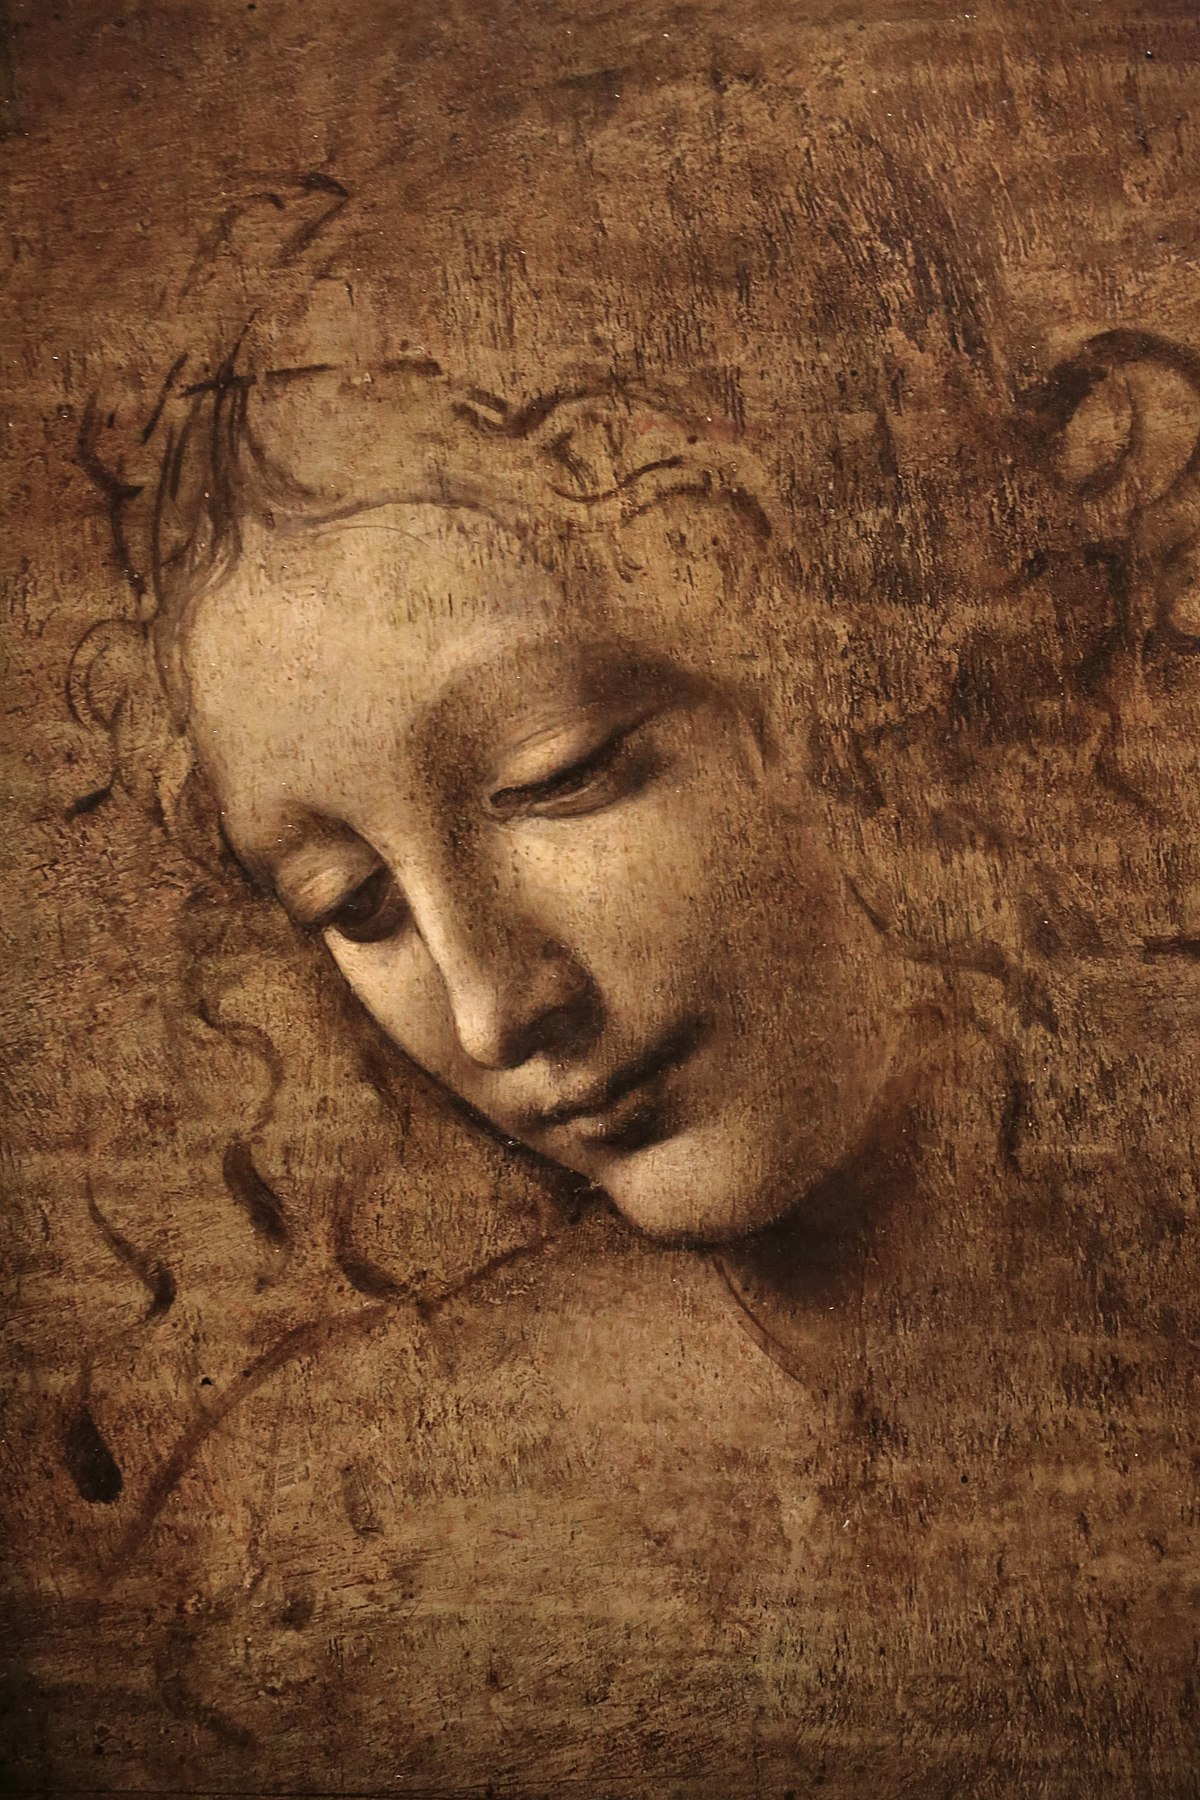
\includegraphics[width=0.4\textwidth]{Figuras/scapigliata}
	\captionsetup{margin=4cm}
	\caption[La Scapigliata]{La Scapiliata, una pintura al oleo sin terminar de fines del Renacimiento. No se conoce el autor, algunos historiadores atribuyen la autoría a Leonardo da Vinci.}
	\label{fig:Scapigliata}
\end{figure}

\LaTeX{} ubica las imágenes dependiendo del espacio que exista en la página. Algunas veces no hay lugar  suficiente para colocar una imagen en donde se declara \verb*|\begin{figure}|, en consecuencia \LaTeX{} la ubica en la parte superior de la siguiente página.
	
	Las figuras deben tener subtítulos los cuales deben ser explicativos y sintéticos.  También se pueden referenciar en el texto (como con la Figura ~ \ref{fig:Scapigliata}). La declaración \verb|\caption| posee dos partes, la primera parte, dentro de los corchetes es el título que aparecerá en el \emph{Índice de figuras}, por lo que debe ser breve. La segunda parte entre llaves debe contener el título más largo y la descripción de la figura. También se puede encuadrar el título de la figura referido al margen de la hoja, para ello debe emplear  \verb*|\captionsetup{margin=4cm}|. 
	
	
	
	También es posible cambiar la posición del comentario, por ejemplo, con la siguiente plantilla de código 
	
	\begin{lstlisting}[basicstyle=\small,tabsize=4]
		\begin{SCfigure}[0.5][h]
			\centering
			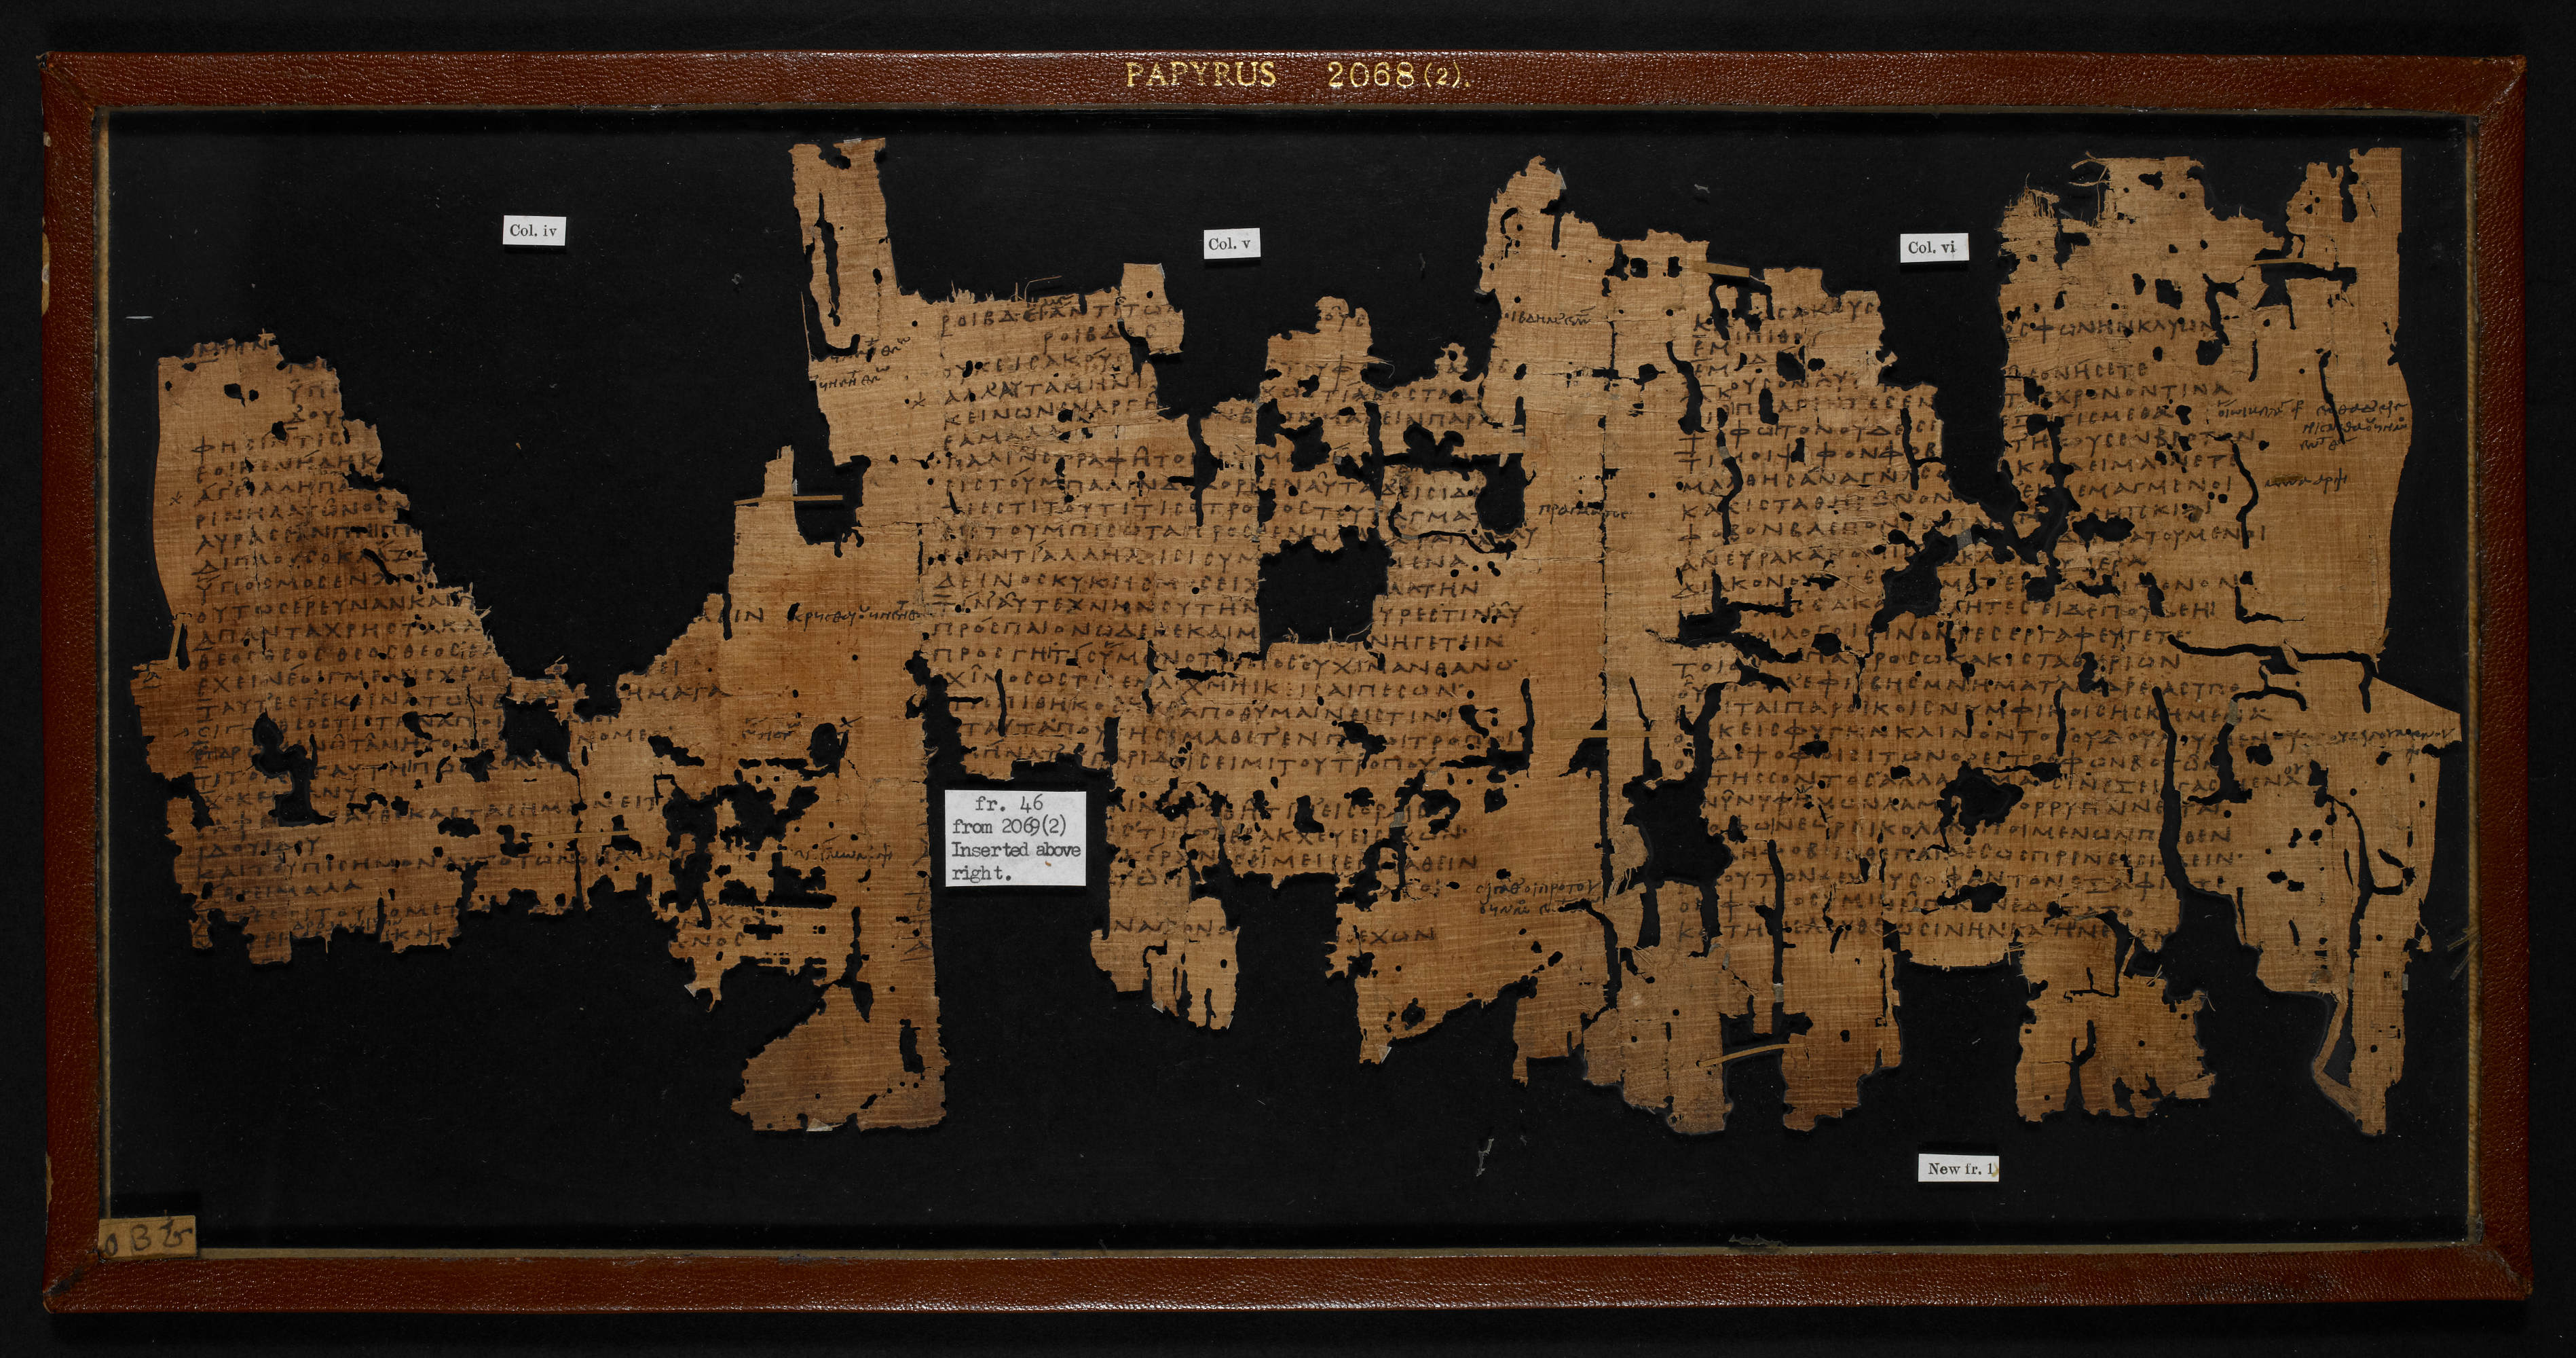
\includegraphics[width=0.6\textwidth]{Figuras/papyrus_sofocles}
			\caption[Ichneutae ....
			\label{fig:diag}
		\end{SCfigure}
	\end{lstlisting}
	
	se obtiene el resultado en la Figura \ref{fig:diag}, donde los comentarios de aparecen a la derecha.
	
	
	\begin{SCfigure}[0.5][h]
		\centering
		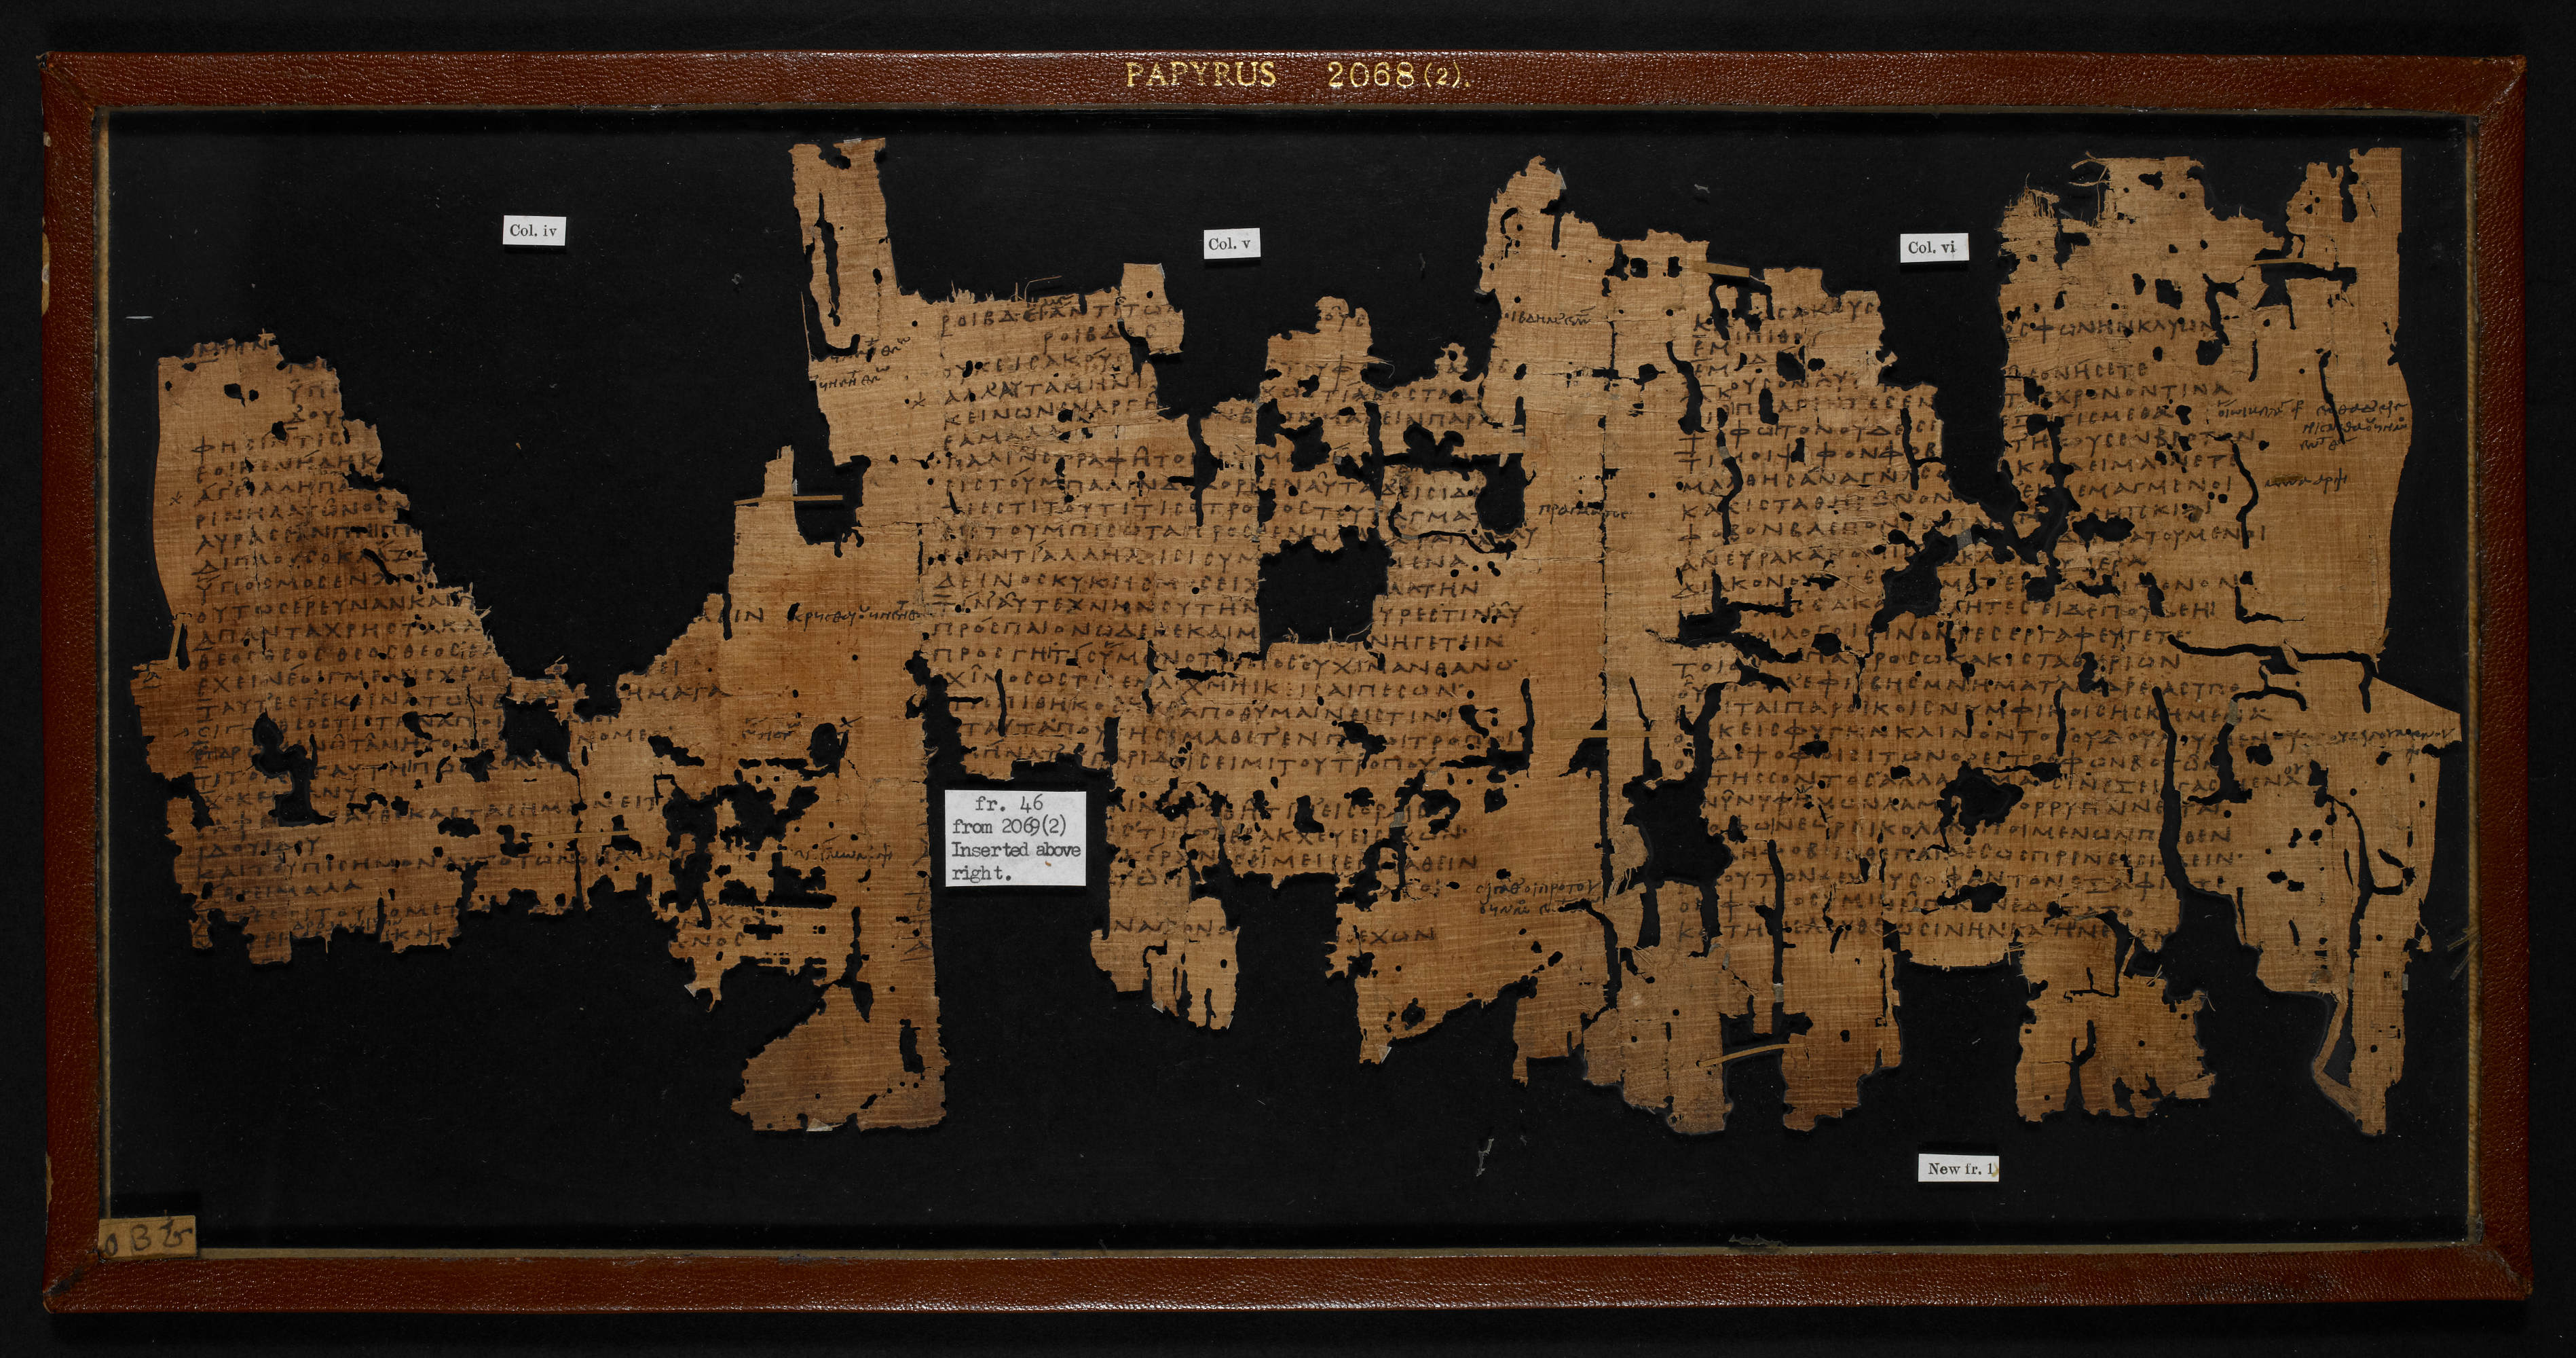
\includegraphics[width=0.6\textwidth]{Figuras/papyrus_sofocles}
		\caption[Ichneutae, o Perseguidores sátiros.]{Ichneutae, o Perseguidores sátiros. Fragmento del manuscrito del dramaturgo ateniense Sófocles. (Museo Británico)}
		\label{fig:diag}
	\end{SCfigure}
	
	%----------------------------------------------------------------------------------------
	\subsection{Una guía corta sobre Algoritmos}
	
	
	\begin{algorithm}[H]
		\label{alg:ejemplo1}
		\SetAlgoLined
		\KwData{$G=(X,U)$ de forma tal que $G^{tc}$ es un orden.}
		\KwResult{Escriba aquí el resultado }
		inicialización\;
		\While{condición}{
			instrucciones\;
			\eIf{condición}{
				instrucción1\;
				instrucción2\;
			}{
				instrucción3\;
			}
		}
		\caption{Cómo escribir una algoritmo}
	\end{algorithm}
	\
	
	Para la escritura de algoritmos existen diferentes posibilidades. En esta plantilla se empleó \verb*|\usepackage{listings}| para mostrar código desde un archivo. \emph{listings} permite listar código en diferentes lenguajes, por ejemplo, en el directorio \file{Codigo} se encuentra el archivo \file{c.c}.
	
	Mediante \verb*|\lstinputlisting[numbers=left, language=c]{Codigo/c.c}| se obtiene
	
	\lstinputlisting[numbers=left, language=c]{Codigo/c.c}
	
	\textbf{Un inconveniente con \emph{listings} es no tener una buena compatibilidad con UNICODE.}
	\\
	
	En muchos casos es preferible presentar un pseudocódigo que muestre en forma genérica la implementación de determinada deducción. Para ello el paquete \emph{algorithm2e} ofrece una alternativa muy conveniente. Se invita a mirar el archivo \file{Capitulos/cap3.tex} para observar el código que permite el resultado del Algoritmo \ref{alg:ejemplo1}
	
	
	
	%----------------------------------------------------------------------------------------

\section{Empiece a trabajar con esta Plantilla}

Si está familiarizado con \LaTeX{}, entonces debería explorar la estructura de directorios de la plantilla y luego proceder a cargar  su propia información en el archivo \file{tesina.tex}.  La sección \ref{CargaArchivo} en la página \pageref{CargaArchivo} le ayudará a hacer esto. Asegúrese de leer también la sección \ref{Convenciones} sobre las convenciones de tesis para aprovechar al máximo esta plantilla.

\subsection{Sobre esta Plantilla.}

Esta plantilla de tesis en \LaTeX{} tiene sus orígenes alrededor de un archivo de estilo \LaTeX{} creado por Steve R.  Gunn de la Universidad de Southampton (Reino Unido), Departamento de Electrónica y Ciencias de la Computación. Puede encontrar el archivo de estilo original en el sitio:
\url{http://www.ecs.soton.ac.uk/~srg/softwaretools/document/templates/}

A su vez, Sunil Patel tomó el archivo de clase \file{ecsthesis.cls} de Steve y lo modificó creando un marco esqueleto y una estructura de carpetas para colocar los archivos de tesis. La plantilla resultante se puede encontrar en el sitio de Sunil aquí: \url{http://www.sunilpatel.co.uk/thesis-template}

Se tomó la plantilla de Sunil, se la simplificó, y se adaptó a la presente plantilla, que conforma el modelo para la Tesina de Licenciatura de Sistemas de la Universidad Nacional de General Sarmiento. 
%----------------------------------------------------------------------------------------

\section{¿Qué incluye esta Plantilla?}

\subsection{Carpetas}
Esta plantilla viene como un único archivo zip que se expande a varios archivos y carpetas. Los nombres de las carpetas son en su mayoría autoexplicativos:

\keyword{Apendices}: esta es la carpeta donde coloca los apéndices. Cada apéndice debe ir en su propio archivo \file{.tex} separado. En el directorio se incluyen un ejemplo y una plantilla.

\keyword{Capítulos}: esta es la carpeta donde se encuentran el resumen y los capítulos de tesis. Una tesis suele tener unos seis capítulos, aunque no existe una regla estricta al respecto. Cada capítulo debe ir en su propio archivo \file{.tex} separado y se pueden dividir como:

\begin{itemize}
	\item \textit{Capítulo 1: Introducción}
	\item \textit{Capítulo 2: Revisión Bibliográfica}
	\item \textit{Capítulo 3: Materiales y Métodos}
	\item \textit{Capítulo 4: Resultados}
	\item \textit{Capítulo 5: Discusión}
	\item \textit{Capítulo 6:Conclusiones y  Recomendaciones}
\end{itemize}


Desde ya esta distribución puede no ser la más conveniente para los trabajos de tesis propuestos, y en ese caso, es conveniente modificarla. 

\keyword{Figuras} -- esta carpeta contiene todas las figuras de interés. En e las imágenes finales que se incluirán en el documento de tesis.

\keyword{Referencias} -- esta carpeta contiene el archivo de referencias bibliográficas \file{.bib}

\keyword{Codigo} -- en esta carpeta debe incluir aquellos archivos de código de programación que le interese mostrar.

\subsection{Archivos}

También se incluyen varios archivos, la mayoría de ellos son texto sin formato y puede ver su contenido en un editor de texto. Después de la compilación inicial, verá que \LaTeX{}  o BibTeX crearán más archivos auxiliares y que no se necesitan eliminar ni preocuparse por ellos.

\keyword{tesina.bib} -- este es un archivo importante que contiene toda la información bibliográfica y referencias que citará en la tesis para su uso con BibTeX. Puede escribirlo manualmente, pero hay programas de administración de referencias disponibles, los cuales permiten crearlo y administrarlo. Las bibliografías en \LaTeX{} son un tema extenso y es posible que deba leer sobre BibTeX antes de comenzar. Muchos sitios de publicaciones científicas y técnicas permiten exportar sus referencias en formato BibTeX, lo que facilita enormemente la compilación que se debe hacer.

\keyword{tesina.pdf} -- esta es su tesis bellamente compuesta (en formato de archivo PDF) creada por \LaTeX {}. Se proporciona  el PDF con la plantilla y, después de compilar la plantilla, debería obtener una versión idéntica.

\keyword{tesina.tex} -- este es un archivo importante. Este es el archivo que le dice a \LaTeX{} que debe compilar para producir su tesis como un archivo PDF. Contiene el marco y las construcciones que le dicen a \LaTeX{} cómo diseñar la tesis. Está muy comentado para que pueda leer lo que hace cada línea de código y por qué está allí. Después de poner su propia información en el bloque \emph{INFORMACIÓN DE TESIS}, ¡ha comenzado su tesis!
\\

Los archivos \emph{no} incluidos, pero creados por \LaTeX{} como archivos auxiliares incluyen:

\keyword{tesina.aux} -- este es un archivo auxiliar generado por \LaTeX{}, si se elimina \LaTeX{} simplemente lo regenera cuando ejecuta el archivo principal \file{.tex}.

\keyword{tesina.bbl} -- este es un archivo auxiliar generado por BibTeX, si se elimina, BibTeX simplemente lo regenera cuando ejecuta el archivo \file{tesina.aux}. Mientras que el archivo \file{.bib} contiene todas las referencias que usted incluyó, el archivo \file{.bbl} contiene las referencias que realmente se han citado en la tesis y se usa para construir la sección de bibliografía de la tesis. \emph{Es posible que cambios en el archivo \file{.bib} no se vean reflejados. Esto se puede deber a que no se recompila el archivo \file{.bbl}, en ese caso, se aconseja borrar al archivo \file{.bbl} para forzar una nueva compilación.}

\keyword{tesina.blg} -- este es un archivo auxiliar generado por BibTeX, si se elimina, BibTeX simplemente lo regenera cuando ejecuta el archivo principal \file{.aux}.

\keyword{tesina.lof} -- este es un archivo auxiliar generado por \LaTeX{}, si se elimina, \LaTeX{} simplemente lo regenera cuando ejecuta el archivo principal \file{.tex}. Le dice a \LaTeX{} cómo construir la sección \emph{Lista de figuras}.

\keyword{tesina.log} -- este es un archivo auxiliar generado por \LaTeX{}, si se elimina \LaTeX{} simplemente lo regenera cuando ejecuta el archivo principal \file{.tex}. Contiene mensajes de \LaTeX{}, si recibe errores y advertencias de \LaTeX {}, estarán en este archivo \file{.log}.

\keyword{tesina.lot} -- este es un archivo auxiliar generado por \LaTeX{}, si se elimina \LaTeX{} simplemente lo regenera cuando ejecuta el archivo principal  file{.tex}. Le dice a \LaTeX{} cómo construir la sección \emph{Lista de tablas}.

\keyword{tesina.out} -- este es un archivo auxiliar generado por \LaTeX{}, si se elimina \LaTeX{} simplemente lo regenera cuando ejecuta el archivo principal  \file{.tex}.

Entonces, de esta larga lista, solo los archivos con las extensiones \file{.bib}  y \file{.tex} son los más importantes. Los otros archivos auxiliares se pueden ignorar o eliminar ya que \LaTeX{} y BibTeX los regenerarán.

%----------------------------------------------------------------------------------------

\section{Cargando la Plantilla con sus datos en  el archivo \file{tesina.tex} }\label{CargaArchivo}


Deberá personalizar la plantilla de tesis y hacerla suya completándola con  su propia información. Esto se hace editando el archivo \file{tesina.tex} en un editor de texto o en su entorno \LaTeX{} favorito.

Abra el archivo y desplácese hacia abajo hasta el tercer bloque grande titulado \emph{DATOS DE PORTADA} donde puede ver las entradas para \emph{Nombre de la Universidad}, \emph{Nombre del Instituto}, etc \ldots

Complete la información sobre usted, grupo e institución. También puede insertar enlaces web, si lo hace, asegúrese de utilizar la URL completa, incluido el código \emph{http://}. Si no desea que estos estén vinculados, simplemente elimine \verb|\href{url}{nombre}| y solo deje el nombre.

\

A continuación se declara la lista de \emph{Acrónimos y Glosario}. Por el repetido uso en el texto de ciertas palabras, o por existir un manera tradicional de escribir una significación, se emplean acrónimos para facilitar la escritura. Son palabras formadas por sílabas o abreviaturas que representan otras palabras y por lo tanto tienen significado. Un ejemplo es \emph{UNGS}, el acrónimo de \emph{Universidad Nacional de General Sarmiento}, otro ejemplo muy común es  \acs{id} (\verb*|\acs{id}|), el cuál significa  \acl{id} (\verb*|\acl{id}|), y se encuentra indicado en la \emph{Lista de Abreviaciones}.  

Por su parte, el \emph{Glosario} es un catálogo alfabetizado de símbolos, palabras y expresiones que son particulares del texto, difíciles de comprender, donde se las lista junto con su significado o algún comentario, por ejemplo , la \emph{densidad superficial de ángeles}, se encuentra definido en el glosario.

En el encabezado de \file{tesina.tex} en el bloque \emph{DECLARACIÓN DE ACRÓNIMOS Y GLOSARIO} se declaran los acrónimos y definiciones que se van a emplear, o no, en el cuerpo de la tesis. Aquellos que se emplearan quedan habilitados para conformar la \emph{Lista de Abreviaciones} y el \emph{Glosario}. 

Estos índices son importantes ya que facilitan al lector la identificación y significado de las abreviaciones que se leen durante el texto. 

\

Cuando haya hecho todas las modificaciones, guarde el archivo y recompile. Toda la información que completó ahora debería estar en el PDF, con los enlaces web. 



%----------------------------------------------------------------------------------------

\section{El archivo \code{tesina.tex} Explicado.}

El archivo \file{main.tex} contiene la estructura de la tesis. Hay muchos comentarios escritos que explican qué páginas, secciones y formato está creando el código \LaTeX{}. Cada elemento principal del documento se divide en bloques comentados con títulos en mayúsculas para que sea obvio lo que está haciendo el  fragmento de código que le sigue. Inicialmente parece haber mucho código \LaTeX{}, pero es declaración de  formato, que ha sido arreglado para que Ud. no tenga que hacerlo.

Luego viene una página que contiene una cita, puede reemplazarla por una cita de su científico, autor, persona, etc. favoritos. Asegúrese de poner el nombre de la persona de quien se tomó la cita.

A continuación, se encuentra la página de \emph{Resumen} que sintetiza su trabajo de manera condensada y casi se puede utilizar como un documento independiente para describir lo que se ha hecho. El Resumen se escribe en el archivo \file{resumen.tex} que se encuentra en la carpeta \emph{Capitulos}


Luego vienen los agradecimientos. En esta página, escriba sobre todas las personas a las que desea agradecer (sin olvidar a los padres, compañeros y a su director y/o supervisor).

Las páginas de contenido, la lista de figuras y las tablas \LaTeX{}  las arma por Ud. en base a la información de estructura que se provee al escribir la tesis, y no es necesario crearlas o editarlas manualmente. En cuanto a la lista de símbolos, abreviaturas y definiciones, debe procurarse que queden ordenadas alfabéticamente, separando alfabetos romanos y griego (esto \emph{no} se hace automáticamente). 

La siguiente página contiene una dedicatoria de una línea. ¿A quién dedicará su tesis?

Finalmente, está el bloque donde se incluyen los capítulos. Elimine el  carácter  \code{\%} para des-comentar las líneas mientras escribe los capítulos. Cada capítulo debe escribirse en su propio archivo, colocarse en la carpeta \emph{Capitulos} y denominarse \file{cap1.tex}, \file{cap2.tex}, etc \ldots De manera similar, para los apéndices, elimine los comentarios de las líneas según los necesite. Cada apéndice debe ir en su propio archivo y colocarse en la carpeta \emph{Apendices}.

Después del preámbulo, capítulos y apéndices finalmente viene la bibliografía. El estilo de bibliografía (llamado \option{plain}) se utiliza para la bibliografía y es un estilo con todas las funciones, e  incluso incluye la posibilidad de  enlaces DOI (así sea agregada en las notas). Su lector estará agradecido al descubrir que una referencia a un artículo está a solo un clic de distancia. Por supuesto, esto depende de que usted ponga la información de la URL en el archivo BibTeX en primer lugar.


%----------------------------------------------------------------------------------------



\section{Conclusión del Capítulo \ref{Cap_Plantilla} }

Ha llegado al final de esta mini-guía. Ahora puede cambiar el nombre o sobrescribir este archivo PDF y comenzar a escribir su propio \file{Capitulo/cap1.tex} y el resto de su tesis.






